\section{Scattering across channels}\label{sec:17.1}

A silicon calorimeter with a threshold of \SI{0.1}{eV} records $3\times10^4$ events per kilogram and year from dark matter of \SI{10}{MeV} that couples to nucleons through a heavy mediator with $\sigma_p = \SI{e-38}{cm^2}$, nearly all of them multiphonon excitations of the lattice. At a threshold of \SI{0.5}{eV} it records 1.5 events, and every one of them is a Migdal ionization. Between the two thresholds the dominant final state moves from the electron-following sector of the decomposition theorem to the two electronic sectors (\cref{sec:8.6}), and the rate drops by four orders of magnitude. For each coupling, the choice of target and threshold depends on where in mass and threshold the dominant sector changes.

\subsection{Kinematic ceilings of the sectors}\label{sec:17.1-ceilings}

At fixed coupling the rate is \cref{eq:8.2-spectrum} with one coupling matrix $\mathfrak{D}$, and by the decomposition theorem \cref{eq:8.6-decomp} the structure factor is the sum of the electron-following, zero-phonon and phonon-dressed sectors. The interference between electrons and nuclei, the bottom row of \cref{tab:8-sectors}, vanishes for a coupling to one species alone (\cref{sec:17.4}). We compare two single-species couplings: a nucleon coupling, with equal couplings to protons and neutrons and the cross-section $\sigma_p$ per nucleon of \cref{sec:11.1}, and an electron coupling with the reference cross-section $\sigmae$. Both couplings have a heavy mediator. The threshold $\omega_{\mathrm{th}}$ acts on the total deposited energy, as in a calorimeter. A charge readout records the electronic sectors alone; the fraction of a lattice deposit that a phonon sensor collects is a question for the chapters on readout.

The first factor that decides the dominant sector is the largest energy that each sector can absorb. A single phonon carries at most the top of the phonon band, \SI{64.1}{meV} in silicon (\cref{sec:5.2}); the PBE density of states used for the maps ends at $\omega_{\mathrm{max}} = \SI{63.7}{meV}$ (\cref{sec:11.3}). A nucleus recoiling freely absorbs at most $E_R^{\mathrm{max}} = 2\mu_{\chi N}^2v_{\mathrm{max}}^2/M$ (\cref{eq:1.3-ERmax}), which is \SI{0.054}{eV} at \SI{10}{MeV} and \SI{5.3}{eV} at \SI{100}{MeV}. An electronic excitation can absorb up to the whole kinetic energy, $\tfrac12\mchi v_{\mathrm{max}}^2$ (\cref{eq:1.3-omegamax}), since the lattice can take the momentum without taking the energy; $\tfrac12\mchi v_{\mathrm{max}}^2$ is \SI{3.5}{eV} at \SI{1}{MeV} and \SI{35}{eV} at \SI{10}{MeV}. For $\mchi \ll M$ the electronic ceiling exceeds $E_R^{\mathrm{max}}$ by the factor $M/4\mchi$, $6.5\times10^3$ at \SI{1}{MeV}. Below the lattice ceiling the electron-following sector dominates whenever the coupling reaches the nuclei, because an electronic excitation costs a small probability per kick. Above it the electronic sectors alone are open. The boundary between the lattice and the electronic regions does not lie exactly at the lattice ceiling, however: a multiphonon spectrum extends above $E_R$ by its Poisson weights, and an impulse peak by its width.

The second factor is screening. A coupling to electrons reaches the lattice through the electrons that move with the nuclei, in full or not at all, according to whether the mediator couples to the electrons alone or to the total charge (\cref{sec:8.4}).

\subsection{Nucleon coupling in silicon}\label{sec:17.1-nucleon}

The nucleon-coupling map uses four responses. Below the zone boundary, $q \le q_{\mathrm{BZ}} = \SI{2.25}{keV}$, the one-phonon response is the long-wavelength acoustic form \cref{eq:11.1-Sac}, with the sound speeds and polarizations of the measured elastic tensor. Since the linear acoustic branches would run above every real phonon near $q_{\mathrm{BZ}}$, we cap the one-phonon deposits at $\omega_{\mathrm{max}}$. Above $q_{\mathrm{BZ}}$ the lattice response is the incoherent harmonic response \cref{eq:11.3-inc}, evaluated with the phonon density of states computed in \cref{sec:5.2} and the Helm form factor of \cref{sec:2.2}, and split into its one-phonon term and the terms with two or more phonons. Above $q = \SI{300}{keV}$, where $2W = 56$, the response is the impulse Gaussian \cref{eq:11.4-IAgauss}. The Migdal rate uses the soft-limit probability \cref{eq:12.3-soft}, evaluated with the loss function with local fields and with the $Z_{\mathrm{ion}}(p)$ of \cref{sec:12.3}. Since the sum rule \cref{eq:12.4-harm} holds at every momentum transfer in its incoherent form (for momentum transfers below $2q_{\mathrm{BZ}}$, see the qualifier on the Migdal band later in this section and \cref{tab:17-nuisances}), the lattice only has to conserve energy, and we give the lattice its mean share of the deposit, $q^2/2M$, so that the deposited energy is $\omega_e + q^2/2M$. The share of Migdal events that leave the lattice in its initial state is $\langle\ee^{-2W(|\vect{q}-\vect{p}|)}\rangle$, averaged, with the weight of \cref{sec:12.4}, over the momentum $\vect{p}$ that the electrons take. We label a point of the map ``one phonon'' when the one-phonon rate above threshold exceeds the rate with two or more phonons. Any other point where the lattice dominates is labeled ``free recoil'' when the median momentum transfer of the lattice rate lies above the impulse onset, \SI{92.5}{keV} (\cref{sec:11.4}). The electron rates are counted from \SI{1.11}{eV}, the gap in the step model of pair creation that is distributed with the loss-function tables. The tables themselves are scissored to the measured gap of \SI{1.17}{eV} (\cref{sec:10.10}), and counting from \SI{1.11}{eV} instead of \SI{1.17}{eV} moves the onset of the electron sector from 0.333 down to \SI{0.316}{MeV}.

\begin{figure}[tbp]
  \centering
  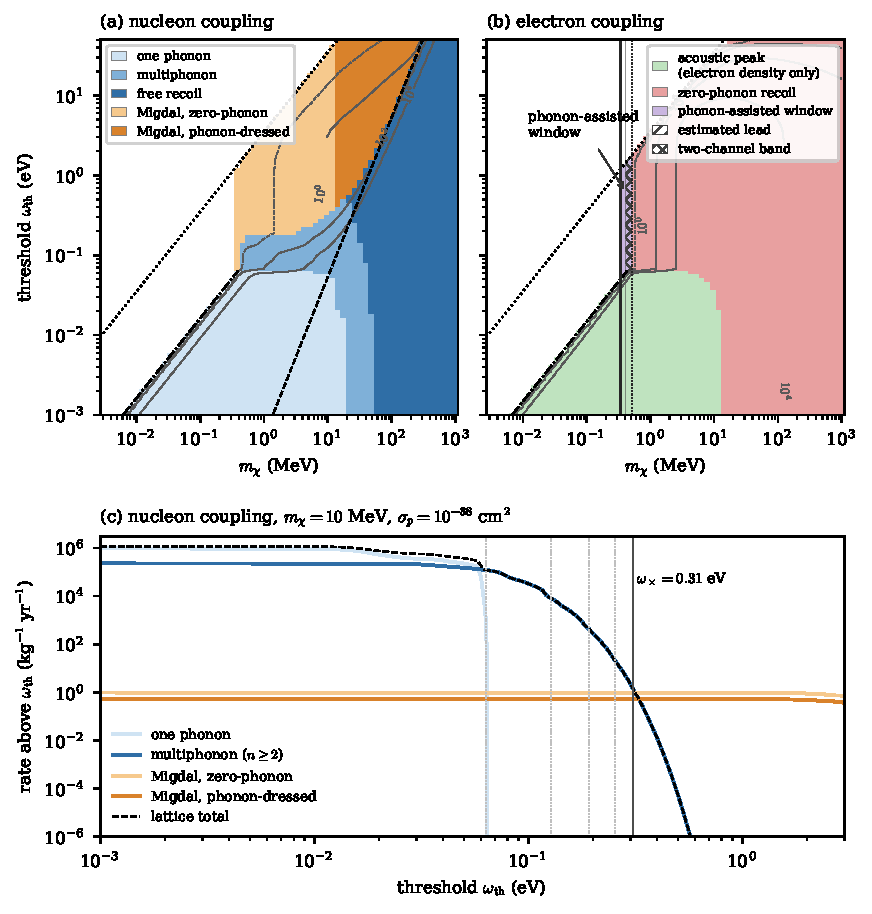
\includegraphics[width=0.86\linewidth]{figures/ch17/fig17_sectors.pdf}
  \caption{Dominant sector of silicon in the plane of dark-matter mass and threshold on the total deposited energy, heavy mediator, standard halo (\cref{tab:1-shm}), $T = 0$. (a)~Nucleon coupling: electron-following sector split into one phonon, two or more phonons and free recoil; Migdal effect split by whether more than half of the events leave the lattice in its initial state; below about \SI{2}{MeV} the Migdal rate carries the unsized coherent factor of \cref{tab:17-nuisances} (at \SI{3}{MeV} the factor acts on \SI{7}{\percent} of the Migdal rate). One-phonon deposits are capped at the top of the PBE band, \SI{63.7}{meV}. Gray contours: the dominant rate, $10^{-2}$ to $10^4$ events per kilogram and year at $\sigma_p = \SI{e-38}{cm^2}$. (b)~Electron coupling: zero-phonon electron recoil (loss function with local fields, counted from \SI{1.11}{eV}) against the acoustic peak of an electron-only coupling (absent for a dark photon) in the model of \cref{lim:10.2a} (linear longitudinal branch to $|\vect{q}| = 2\pi/a$, 28 electrons per cell following the nuclei). Phonon-assisted window from \cref{tab:13-window}: onsets 0.3332 (dashed) and \SI{0.3374}{MeV} (solid) and first zero-phonon edge 0.405--\SI{0.408}{MeV} (dark band), computed; estimated phonon-assisted lead to \SI{0.43}{MeV} (hatched) and two-channel band 0.43--\SI{0.51}{MeV} (cross-hatched). Contours at $\sigmae = \SI{e-37}{cm^2}$. Lines: dotted, the largest deposit $\tfrac12\mchi v_{\mathrm{max}}^2$; dashed, the free-recoil endpoint $E_R^{\mathrm{max}}$; dash-dotted, the acoustic edge \cref{eq:11.1-edge} with $c_{\mathrm{LA,max}} = \SI{9.35}{km/s}$ in (a) and the model's \SI{8.43}{km/s} in (b). White: no channel, or a rate below $10^{-12}$ events per kilogram and year. (c)~Rates above threshold at $\mchi = \SI{10}{MeV}$, nucleon coupling; vertical dotted lines at multiples of the band top, solid line at the crossover threshold $\omega_{\mathrm{th}}^\times$ of \cref{we:17-crossover}.}
  \label{fig:17-sectors}
\end{figure}

\Cref{fig:17-sectors}a shows the result. Below the band top the electron-following sector holds the whole map, and inside it the one-phonon term leads up to \SI{20}{MeV} at a threshold of \SI{1}{meV}, although the kicks of a \SI{10}{MeV} particle already reach $2W = 1.8$. The reason is that the incoherent response gives the one-phonon term the Poisson weight $2W\ee^{-2W}$, and the sum of all higher orders overtakes the one-phonon weight only at $2W = 1.26$. The heavy mediator weights the largest momentum transfers, so the boundary of the one-phonon region follows the typical kick. Below \SI{3.4}{MeV}, where $q_{\mathrm{max}} < \SI{18}{keV}$, the one-phonon contours carry the coherent correction of \cref{sec:11.3}, which exceeds \SI{10}{\percent} below \SI{18}{keV}; the boundary of the one-phonon region near \SI{20}{MeV}, where the kicks lie far above \SI{18}{keV}, does not. Multiphonon deposits dominate above \SI{20}{MeV} at the lowest thresholds and, at every mass, at thresholds above the band top. By the median criterion the free recoil leads above \SI{60}{MeV} at \SI{1}{meV}, and above \SI{22}{MeV} at higher thresholds. At the lowest thresholds the lattice rate exceeds the Migdal rate by roughly the inverse of the Migdal probability per kick, averaged over the kicks: by $6\times10^7$ at \SI{1}{MeV}, $8\times10^5$ at \SI{10}{MeV} and $2\times10^4$ at \SI{100}{MeV}.

\begin{table}[tbp]
  \caption{The multiphonon--Migdal crossover in silicon: nucleon coupling, heavy mediator, $\sigma_p = \SI{e-38}{cm^2}$, threshold on the total deposited energy. Largest momentum transfer and its Debye--Waller exponent; crossover threshold $\omega_{\mathrm{th}}^\times$ (lattice rate equal to the Migdal rate) and its ratio to the free-recoil endpoint; Migdal rate at the lowest thresholds (events per kilogram and year) and its zero-phonon share.}
  \label{tab:17-crossover}
  \centering\small
  \begin{tabular}{@{}lccccccc@{}}
    \toprule
    $\mchi$ (MeV) & 1 & 3 & 6.3 & 10 & 17.5 & 30 & 100 \\
    \midrule
    $q_{\mathrm{max}}$ (keV) & 5.3 & 15.9 & 33.4 & 53.0 & 92.7 & 159 & 528 \\
    $2W(q_{\mathrm{max}})$ & 0.02 & 0.16 & 0.70 & 1.76 & 5.40 & 15.9 & 175 \\
    $\omega_{\mathrm{th}}^\times$ (eV) & 0.178 & 0.187 & 0.242 & 0.307 & 0.466 & 0.826 & 5.33 \\
    $\omega_{\mathrm{th}}^\times/E_R^{\mathrm{max}}$ & 331 & 38.8 & 11.3 & 5.73 & 2.84 & 1.71 & 1.00 \\
    Migdal rate & $1.9\times10^{-3}$ & 0.12 & 0.68 & 1.5 & 3.4 & 6.9 & 30 \\
    zero-phonon share & 0.97 & 0.94 & 0.83 & 0.65 & 0.33 & 0.10 & 0.001 \\
    \bottomrule
  \end{tabular}
\end{table}

The Migdal effect holds the band between the end of the lattice spectrum and the largest deposit. The Migdal band opens at a mass of $2\Eg/v_{\mathrm{max}}^2$. Up to \SI{1}{MeV} the Migdal rate comes from momentum transfers between about \SI{0.75}{keV} and $2q_{\mathrm{BZ}}$, where the diagonal soft limit of \cref{sec:12.4} is not known to equal the coherent response and the coherent response is not computed. Near threshold the factor that takes the diagonal soft limit to the coherent response is likely a large suppression, since the exact small-$q$ spectrum lies at the plasmon, beyond the energies that are open near threshold. The Migdal band at 0.32--\SI{1}{MeV} carries this unsized coherent factor, and so does the \SI{1}{MeV} column of \cref{tab:17-crossover}, since the whole Migdal rate at \SI{1}{MeV} comes from momentum transfers between about \SI{0.75}{keV} and $2q_{\mathrm{BZ}}$ (\SI{29}{\percent} of it from below $q_{\mathrm{BZ}}$). At \SI{2}{MeV} the coherent factor acts on a third of the Migdal rate, and from \SI{3}{MeV} on, on \SI{7}{\percent} or less (\cref{tab:17-nuisances}). \Cref{tab:17-crossover} gives the crossover threshold $\omega_{\mathrm{th}}^\times$, where the lattice and the Migdal rates are equal. Below \SI{3}{MeV} the kicks are soft, $2W(q_{\mathrm{max}}) \le 0.16$, and the crossover stays near $2.8$ to $2.9\,\omega_{\mathrm{max}}$. A deposit above $2\omega_{\mathrm{max}}$ needs three phonons, and the three-phonon weight scales as $(2W)^3$, against $2W$ for the Migdal probability; the three-phonon spectrum falls so steeply at its top that a smaller $2W$ moves the crossover little. Between 3 and \SI{20}{MeV} the crossover climbs through the Poisson tail of the multiphonon spectrum, as \cref{we:17-crossover} works out at \SI{10}{MeV}. Above the impulse onset the lattice deposit is a peak at $E_R$ with a Gaussian tail, and the crossover moves onto the free-recoil endpoint. At \SI{300}{MeV} it lies at $0.98\,E_R^{\mathrm{max}}$, below the endpoint, because $\eta(\vmin)$ vanishes at the endpoint faster than the Migdal rate falls. Above \SI{410}{MeV} the endpoint passes the \SI{89}{eV} end of the tables, and the Migdal side of the map would need the core shells (\cref{sec:12.2}). Inside the Migdal band a charge readout at the single-electron level records the Migdal events with no lattice background from the dark matter itself.

The Migdal region of \cref{fig:17-sectors}a splits at one mass into a zero-phonon and a phonon-dressed part. A zero-phonon Migdal event needs the lattice to absorb the kick coherently, with probability $\ee^{-2W}$ at the momentum the nucleus keeps. The rate-weighted share of zero-phonon events falls with mass (\cref{tab:17-crossover}), and it equals the phonon-dressed share at \SI{13.2}{MeV}. This crossing lies above the \SI{6.3}{MeV} at which a kick at the largest momentum transfer gives $\ee^{-2W} = \tfrac12$ (\cref{sec:12.4}), since the halo puts most kicks below the largest one. At \SI{300}{MeV} the Migdal rate at the lowest thresholds reaches 130 events per kilogram and year.

\begin{workedexample}{The multiphonon--Migdal crossover in silicon at 10 MeV}\label{we:17-crossover}
\emph{Kinematics.} For $\mchi = \SI{10}{MeV}$ the largest momentum transfer is $q_{\mathrm{max}} = 2\mu_{\chi N}v_{\mathrm{max}} = \SI{53.0}{keV}$, and a free recoil there would take $E_R^{\mathrm{max}} = \SI{53.7}{meV}$. With the mean phonon energy $\langle\omega\rangle = \SI{40.9}{meV}$ the recoil parameter of \cref{sec:8.5} is $x_R = E_R/\langle\omega\rangle = 1.31$, below the impulse onset $x_R = 4$ (\cref{sec:11.4}). The lattice therefore takes the energy in whole phonons, with Poisson weights of mean $2W = q^2\langle u_x^2\rangle = 1.76$, where $\langle u_x^2\rangle = \SI{2.45e-3}{\angstrom^2}$ is the mean square displacement of \cref{sec:11.3}.

\emph{Migdal side.} The Migdal probability per kick is $6.07\times10^{-5}$ per eV of recoil energy (\cref{sec:12.3}), or $3.26\times10^{-6}$ at $q_{\mathrm{max}}$, all of it at $\omega_e \ge \SI{1.11}{eV}$.

\emph{Lattice side.} The incoherent spectrum at $q_{\mathrm{max}}$ is $8.1\times10^{-3}$ per eV at \SI{0.3}{eV}, where seven phonons give \SI{35}{\percent} of it, and $1.24\times10^{-4}$ per eV at \SI{0.4}{eV}, a fall by a factor 65 per \SI{0.1}{eV}. The weight above \SI{0.4}{eV} is then $1.24\times10^{-4} \times \SI{0.024}{eV} = 3.0\times10^{-6}$, equal to the Migdal probability: per kick, the crossover lies near \SI{0.4}{eV}.

\emph{Rates.} Integrated over momentum transfer and halo, the lattice rate above 0.1, 0.2, 0.3 and \SI{0.5}{eV} is $3.3\times10^4$, 283, 2.2 and $5.5\times10^{-5}$ events per kilogram and year at $\sigma_p = \SI{e-38}{cm^2}$, against a Migdal rate of 1.5 (0.98 zero-phonon, 0.53 phonon-dressed) that does not change below \SI{1.1}{eV}. The lattice and Migdal rates are equal at $\omega_{\mathrm{th}}^\times = \SI{0.307}{eV}$, or $5.7\,E_R^{\mathrm{max}}$ and $4.8\,\omega_{\mathrm{max}}$. The rate crossover lies below the per-kick value because softer kicks lose more of their tail than of their Migdal probability: the tail scales as a high power of $2W \propto q^2$, the Migdal probability as $q^2$. Near $\omega_{\mathrm{th}}^\times$ the lattice rate falls by a factor $e$ every \SI{0.020}{eV}. The coherent corrections to multiphonon spectra near their band edges are about a factor of two in the tail (\cref{sec:11.3}), and a change of that size moves $\omega_{\mathrm{th}}^\times$ by \SI{0.014}{eV}.
\end{workedexample}

\subsection{Electron coupling and screening}\label{sec:17.1-electron}

An electron coupling reaches the zero-phonon, phonon-dressed and electron-following sectors of silicon. The zero-phonon sector gives the loss-function rate \cref{eq:10.2-rate}, open above the first zero-phonon edge at 0.405 to \SI{0.408}{MeV}, and we evaluate this rate with the loss function with local fields. The phonon-dressed sector gives the phonon-assisted rate of \cref{sec:13.3}, open from 0.3332 or \SI{0.3374}{MeV}; for the window between the phonon-assisted onset and the zero-phonon edge we take \cref{tab:13-window}, where only estimates of the phonon-assisted rate exist. The electron-following sector gives the acoustic peak of \cref{sec:10.2}, carried by the electrons that move with the nuclei. We evaluate the acoustic peak in the model of \cref{lim:10.2a}: a linear longitudinal branch with $c_{\mathrm{LA}} = \SI{8.43}{km/s}$ up to $|\vect{q}| = 2\pi/a = \SI{2.28}{keV}$, where the branch reaches \SI{64}{meV}, and all 28 electrons of the cell following the nuclei.

\Cref{fig:17-sectors}b shows the map. Below \SI{0.3332}{MeV} the acoustic peak is the one open channel, and it is open up to its top at \SI{64}{meV}. Between 0.3332 and \SI{0.405}{MeV} the phonon-assisted channel is the one electronic channel; by the estimates of \cref{sec:13.9} it leads centrally to \SI{0.43}{MeV}, the phonon-assisted and zero-phonon channels are comparable from 0.43 to \SI{0.51}{MeV}, and above \SI{0.51}{MeV} the zero-phonon rate leads. Wherever the acoustic peak is open, it dominates the low thresholds: it exceeds the electron-recoil rate by $4.4\times10^4$ at \SI{1}{MeV} and by 1.2 at \SI{10}{MeV}, and the two rates are equal at \SI{12.3}{MeV}, above which the electron recoil leads at every threshold. The crossing at \SI{12.3}{MeV} is a property of the model, however. In the model the acoustic peak stops at \SI{2.28}{keV}, a momentum transfer that dark matter of \SI{0.43}{MeV} already reaches, and above that mass the peak falls as $1/(\mchi\mu_{\chi e}^2)$, while the electron recoil keeps gaining phase space at large $q$ up to \SI{10}{MeV}. Umklapp terms, the transverse branches and the multiphonon deposits of the following charge are all absent from the model and would add to the peak; the bending of the dispersion and the loss of following charge at finite $q$ would take from the peak (\cref{sec:10.2}).

Screening decides which of the low-threshold regions exists. For a coupling proportional to the total charge, as for a dark photon, the exactness theorem \cref{eq:8.4-exact} makes $S_{ZZ}$ proportional to the loss function at every $(q,\omega)$ with the nuclei free to move. The loss function of silicon has no acoustic peak at order $q^2$: the Born charges vanish, so the electrons that follow a displaced nucleus cancel its charge, and the acoustic weight of $S_{ZZ}$ starts at order $q^4$ (\cref{sec:8.4}). For a dark photon the green region of \cref{fig:17-sectors}b is empty to the order computed in this book, and silicon below \SI{0.3332}{MeV} has no channel. For a mediator that couples to the electrons alone, on the other hand, nothing cancels the following charge. The following charge holds a share of just $Z_\kappa m_e/M_\kappa = 2.73\times10^{-4}$ of the $f$-sum (\cref{sec:8.6}), but that share lies at phonon energies, where the electronic sectors have no weight. As a result the rate at \SI{1}{MeV} grows from 17 to $7\times10^5$ events per kilogram and year at $\sigmae = \SI{e-37}{cm^2}$. Above the gap the rates of a total-charge coupling and of an electron-only coupling differ by the ratio of the electron-only loss function to the total loss function. The ratio equals one at clamped nuclei, and above the phonon band it equals one to the order of the Migdal effect (\cref{sec:8.4}). In silicon, then, a detector that probes the electron coupling below the gap tests whether the mediator couples to the total charge or to the electrons alone. A nucleon coupling is unscreened at phonon energies in silicon for the same reason that the dark photon is screened away: the nucleon vertex is not the charge, and the vanishing Born charges remove its one screening term (\cref{sec:8.4}).

\subsection{Germanium and GaAs}\label{sec:17.1-ge-gaas}

In germanium and GaAs the silicon maps change through the sector edges collected in \cref{tab:17-boundaries}. Germanium is heavier and softer. Its acoustic edge lies above silicon's, and its phonon-assisted onset lies below silicon's because the gap of germanium is smaller (\cref{tab:9-edges}). The zero-phonon edge of germanium, however, is not known (\cref{sec:13.9-ge-gaas}), so the electron-coupling map of germanium has an open boundary where silicon's has a computed one. In the nucleon-coupling map of germanium the zero-phonon Migdal region reaches a higher mass, with $\ee^{-2W} = \tfrac12$ at \SI{7.7}{MeV}, and the impulse onset lies at \SI{21.3}{MeV}; both masses come from an estimated mean phonon frequency (\cref{sec:12.4,sec:11.4}). Since the phonons of germanium are softer, with a Debye temperature of \SI{373}{K} against \SI{645}{K} (\cref{sec:11.1}), a deposit of given energy needs more phonons, and the Migdal band should begin at a lower threshold than in silicon at the same mass.

GaAs shows what screening does when the Born charges do not vanish. A dark photon couples to the longitudinal optical phonon of GaAs through $Z^* = 2.11$ (\cref{sec:11.2}). The polar one-phonon rate opens at $2\omega_{\mathrm{L}}/v_{\mathrm{max}}^2 = \SI{10.35}{keV}$ with $\omega_{\mathrm{L}} = \SI{36.35}{meV}$ and, for a light mediator at $\sigmae = \SI{e-40}{cm^2}$, rises to 840 events per kilogram and year near \SI{29}{keV} (\cref{fig:11-polar}). Below the gap the total-charge map of GaAs is filled by the electron-following sector, where silicon's is empty. The electronic sectors open at \SI{0.433}{MeV}, the kinematic floor of the direct gap, where a phonon must still take the momentum (\cref{sec:9.2-mmin}). The phonon-assisted channel leads from 0.433 to between 0.52 and \SI{0.56}{MeV}, where the L valleys open the zero-phonon channel (\cref{sec:13.1}). A nucleon coupling, by contrast, barely sees the polar mode. Its vertex on the optical phonon at small $q$ is set by the difference between the two sublattices in the mean nucleon number per mass: 1.001072 per u for gallium and 1.001046 per u for arsenic, a difference of $2.59\times10^{-5}$ per u (\cref{we:8-nucleon}). At finite $q$ the relative phase of the two sites adds to this vertex, and the map of a nucleon coupling in GaAs has the structure of silicon's, with acoustic, multiphonon and Migdal regions.

\begin{table}[tbp]
  \caption{Edges of the dominant-sector map in silicon, germanium and GaAs, heavy mediator, standard halo. Masses in MeV unless marked. Status: computed (one or two calculations), measured data, estimate, or a property of a model, as marked in each cell. The kinematic floor, the acoustic edge and the impulse onset of the three crystals are in \cref{tab:9-edges}.}
  \label{tab:17-boundaries}
  \centering\footnotesize\setlength{\tabcolsep}{3pt}
  \begin{tabular}{@{}>{\raggedright\arraybackslash}p{0.31\linewidth}>{\raggedright\arraybackslash}p{0.2\linewidth}>{\raggedright\arraybackslash}p{0.2\linewidth}>{\raggedright\arraybackslash}p{0.21\linewidth}@{}}
    \toprule
    Edge & Si & Ge & GaAs \\
    \midrule
    Lattice sector of a dark photon below the gap & none at order $q^2$ ($Z^* = 0$) & none at order $q^2$ ($Z^* = 0$) & polar phonon from \SI{10.35}{keV} \\
    Phonon-assisted onset & 0.3332 (replica), 0.3374 (free pair); one calculation & 0.2119--0.2141; measured data & 0.433--0.436; estimate \\
    Zero-phonon electronic edge & 0.405--0.408; two calculations & open & L channel 0.517--0.560 ($\mathrm{\Gamma}$ pair closed) \\
    Phonon-assisted rate leads & to $\approx 0.43$; estimate & open & to 0.52--0.56; estimate \\
    $\ee^{-2W} = \tfrac12$ at $q_{\mathrm{max}}$ & 6.3 & $\approx 7.7$; estimate & not evaluated \\
    Multiphonon--Migdal crossover at \SI{10}{MeV} & \SI{0.307}{eV} (\cref{tab:17-crossover}) & not evaluated & not evaluated \\
    Acoustic peak of an electron-only coupling $=$ electron recoil, $\omega_{\mathrm{th}} = \SI{1}{meV}$ & 12.3; property of the model & not evaluated & not evaluated \\
    \bottomrule
  \end{tabular}
\end{table}

The maps are limited first by the electron-following sector of an electron-only coupling, which is known in silicon only as the long-wavelength model of \cref{sec:10.2}. To fix the mass above which electron recoil dominates the low thresholds, we would need a calculation of the density that follows the nuclei at momentum transfers up to several times the zone, with Umklapp and multiphonon terms. The phonon-assisted side of the window is an estimate known to a factor of ten; computing the phonon-assisted rate from the amplitude, on the same bins as the zero-phonon rate, would turn the hatched bands into computed boundaries. Germanium lacks a known zero-phonon edge and, beyond the Debye estimate of \cref{sec:5.3}, a computed phonon density of states, so neither the electronic window nor the multiphonon--Migdal crossover of germanium can be drawn. The crossover in silicon is insensitive to the shape of the multiphonon tail, but it inherits from the Migdal probability the factor 1.35 of local fields and the open off-diagonal correction (\cref{sec:12.3}); together they move the crossover by \SI{0.006}{eV} at \SI{10}{MeV}.
